\chapter{Introduction}
\label{chap:intro}

\begin{flushright}
\begin{small}
\textit{Even in science, the object of research is no longer nature itself, but man's investigation of nature.}\\
Werner Heisenberg
\end{small}
\end{flushright}

\section{On the importance of glaciers}

Glaciers are fascinating natural systems to study. Their beauty originates from complex interactions between climate and topography, creating  unique natural features that shape landscapes, influence ecosystems and even climates wherever they flow. These perennial ice masses originate in places allowing the accumulation of snow, that over the course of years gradually transform into firn and eventually ice. Due to gravity, this ice flows downwards, reaching lower elevations with higher temperatures where ice is lost through different processes of ablation, such as ice melting or calving \citep{ipcc_climate_2018}. The sum of all accumulation and ablation in a glacier determines its mass balance, which is essential to monitor the evolution of glaciers through time and their contribution to sea level rise (Fig. \ref{intro:fig1}). Glaciers are excellent climate proxies, adjusting their geometry and size to changes in climate. They represent a large part of the cryosphere, covering some 10\% of the Earth's land surface and storing about 69\% of the world's fresh water \citep{cuffey_physics_2010}. In their study, glaciers are often divided into mountain glaciers (Fig. \ref{intro:fig1}) and ice-sheets, which differ in size and geographical location, with ice-sheets being much larger than mountain glaciers and situated in Greenland and Antarctica \citep{benn_glaciers_2014}.  

Mountains are the water towers of the world, acting as buffers that store solid precipitation and distribute fresh water resources throughout the year \citep{immerzeel_importance_2020}. Seasonal and long-term cryospheric changes in mountain environments regulate water, nutrient and sediment supply downstream \citep{huss_toward_2017}. Glaciers play a major role in this, providing water resources during the warmest or driest months well after all snow has melted. This late summer runoff is essential to many ecosystems requiring cold water and humid habitats throughout the year \citep{cauvy-fraunie_global_2019, carlson_monitoring_2020}. About 10\% of the global population live in mountain areas and the contiguous plains, depending on these water resources for agriculture, industry, hydropower, recreation activities or domestic use \citep{huss_global-scale_2018,farinotti_large_2019}. Mountain areas are amongst the most affected regions by anthropogenic climate change, outpacing global warming  with an increase of +0.3ºC per decade \citep{ipcc_climate_2018}. These rapid changes in climate are causing a widespread retreat of glaciers (Fig. \ref{intro:fig1}), with many regions already having reached "peak water", i.e. the maximum glacier runoff. Once this point is reached, glaciers progressively reduce their water contributions, altering the hydrological regime of glacierized watersheds \citep{huss_global-scale_2018}. The disappearance of glaciers produces an early release of accumulated solid precipitation in spring and early summer, with potential droughts in late summer \citep{brunner_future_2019}. This represents a transition from a nivo-glacial hydrological regime towards a nival hydrological regime. These fast changes in mountain glaciers also result in glaciers currently being important contributors to sea level rise (0.92 $\pm$ 0.39 mm a$^{-1}$), as much as the massive Antarctic and Greenland ice-sheets combined over the 20$^{th}$ century, despite representing less than 1\% of the ice on Earth \citep{zemp_global_2019, hock_glaciermip_2019}. 

\begin{figure*}[h]
\centering
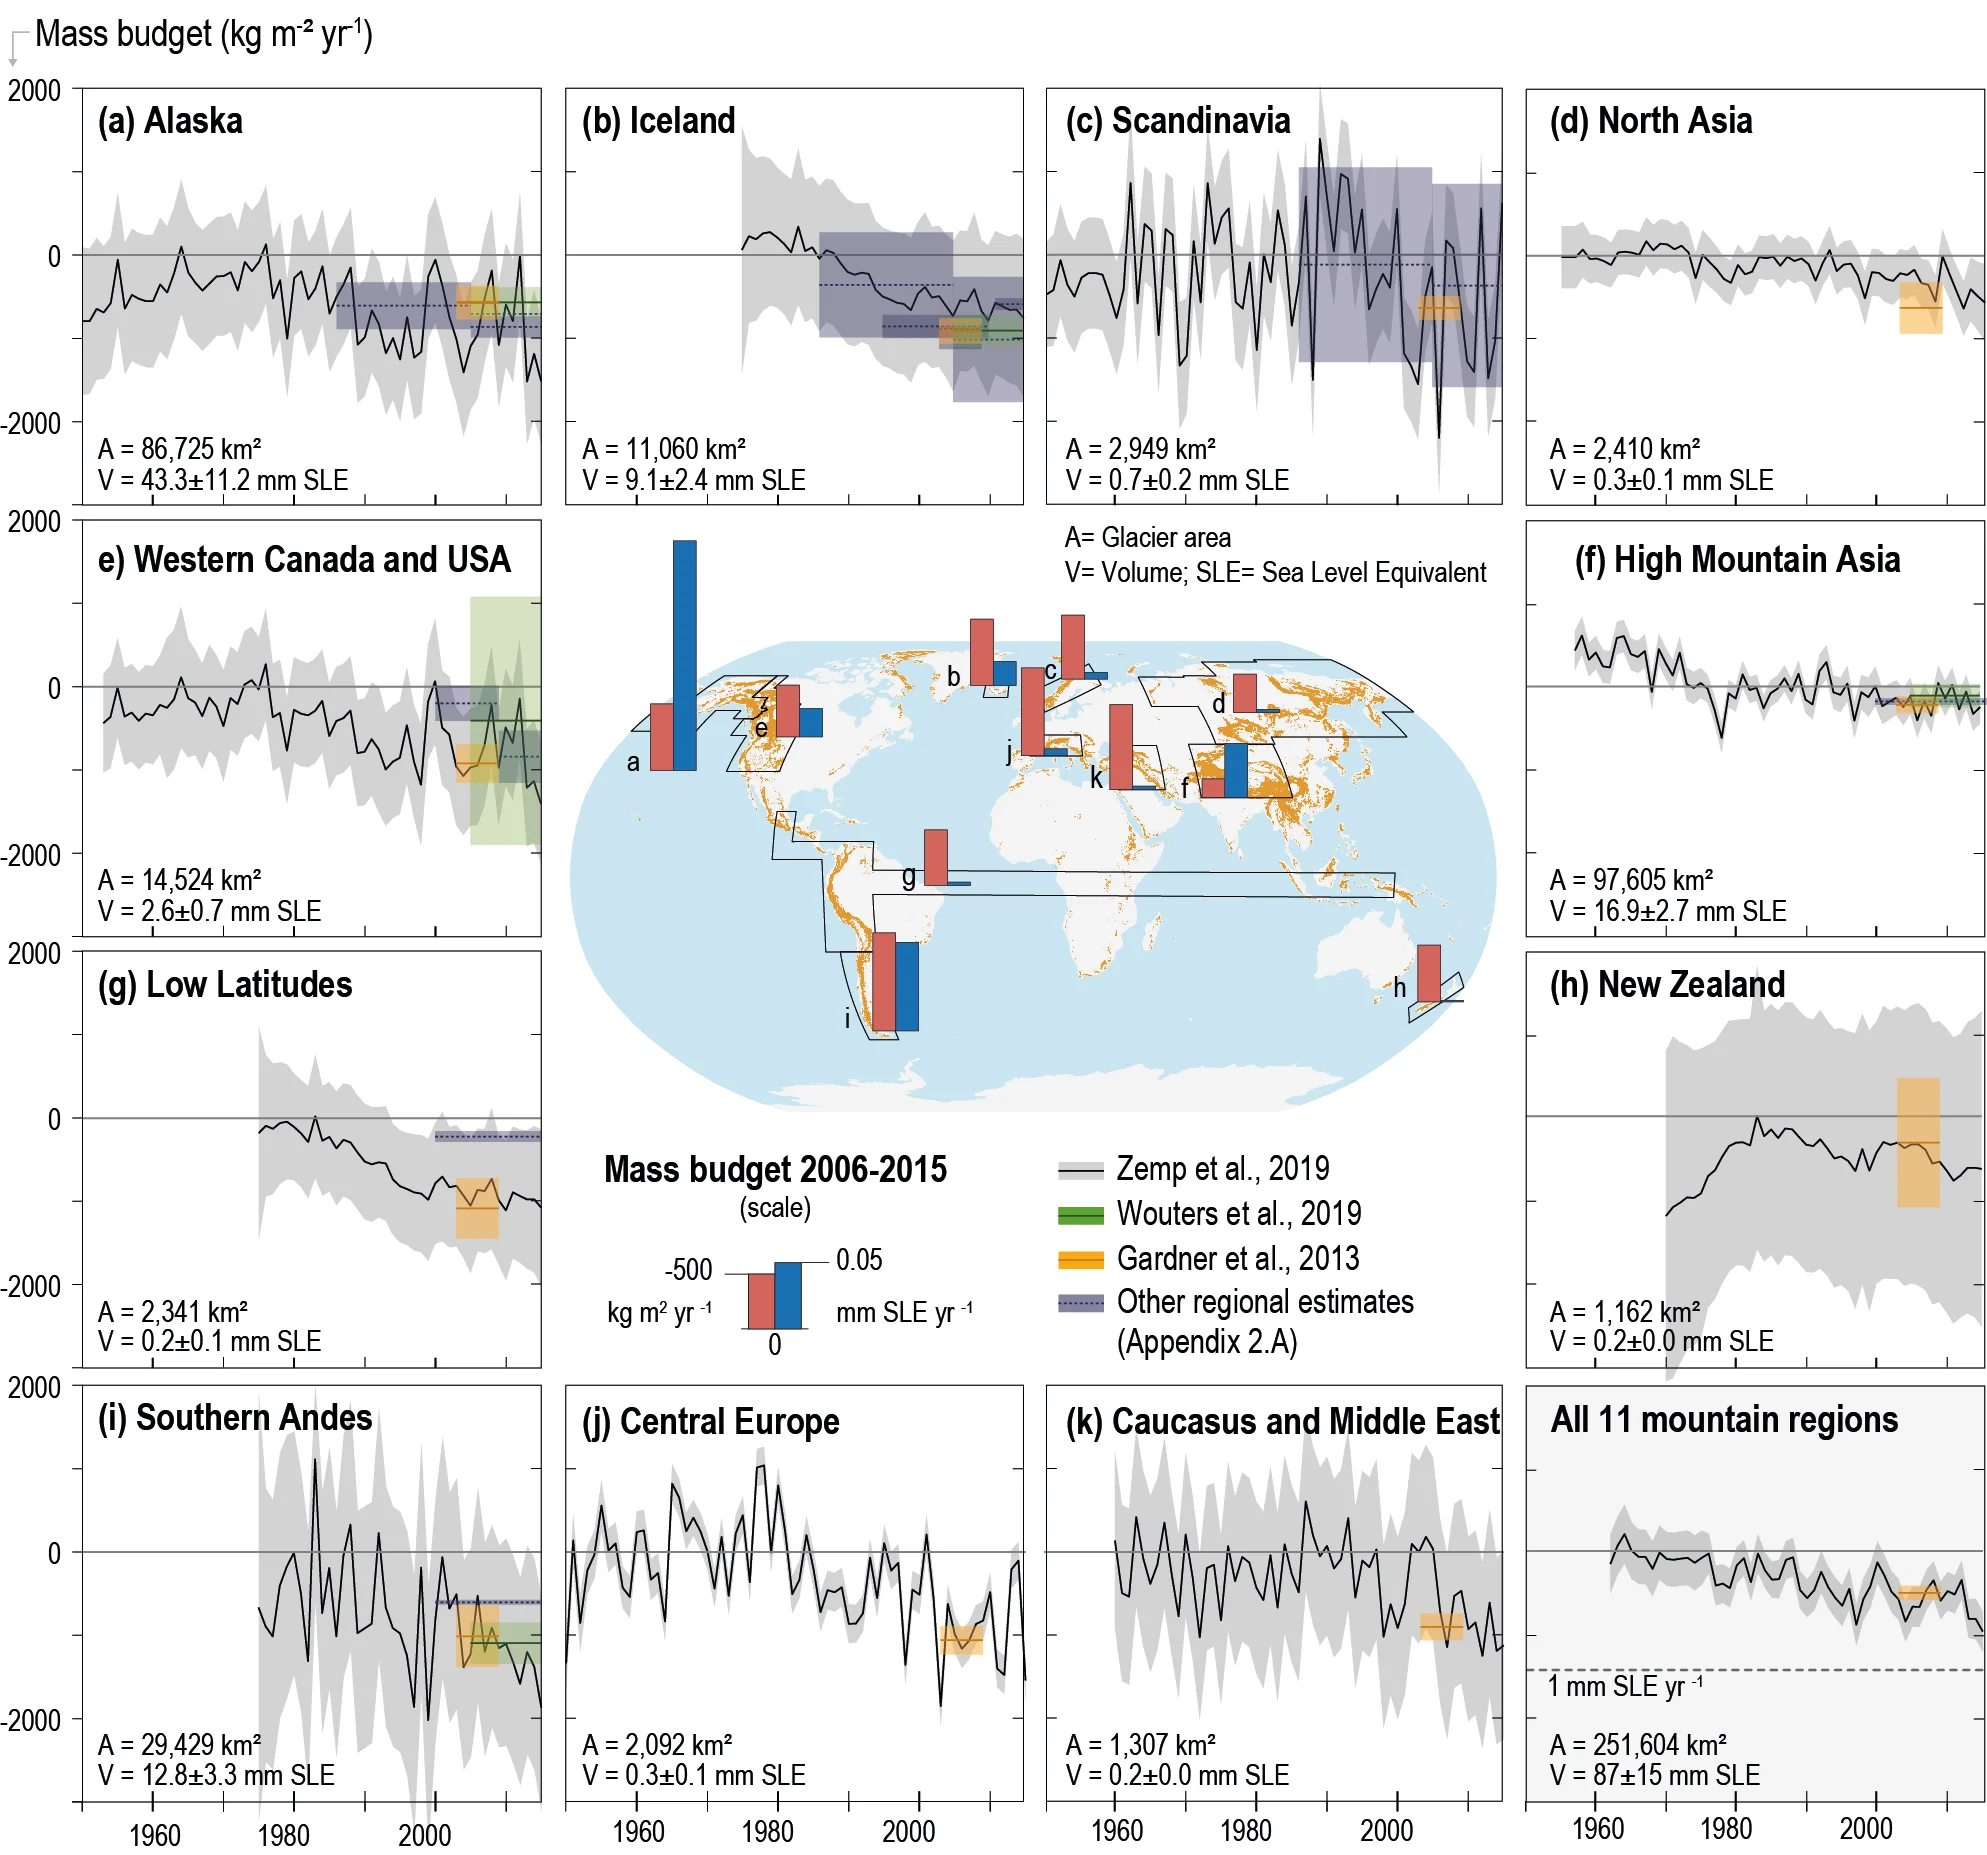
\includegraphics[width=14cm]{Figures/intro/Figure_1.png}
\caption{Glacier mass budgets for eleven different mountain regions and their combined results. Regional time series of annual mass change are based on glaciological and geodetic balances (Zemp et al., 2019). Superimposed are multi-year averages by Wouters et al. (2019) based on the Gravity Recovery and Climate Experiment (GRACE), only shown for the regions with glacier area > 3,000 km$^{2}$. Estimates by Gardner et al. (2013) were used in the IPCC 5th Assessment Report (AR5). Annual and time-averaged mass-budget estimates include the errors reported in each study. Glacier areas (A) and volumes (V) are based on RGI Consortium (2017)
and Farinotti et al. (2019), respectively. Red and blue bars on map refer to regional budgets averaged over the period 2006–2015 in units of kg m$^{–2}$ a$^{–1}$ and mm sea level equivalent (SLE) a$^{–1}$, respectively, and are derived from each region's available mass-balance estimates. \textit{Figure from IPCC's Special Report on the Ocean and Cryosphere in a Changing Climate (SROCC, 2019).}} 
\label{intro:fig1}
\end{figure*}

Mountain glaciers are predicted to lose an important fraction of their overall mass by the end of the 21$^{st}$ century, with great differences between regions \citep{hock_glaciermip_2019}. An accurate assessment of future glacier evolution is essential to understand and quantify the environmental and social consequences of their retreat. Since glaciers have become an icon of climate change, accurate predictions paired with effective communication can prove a great way to raise awareness on climate change. Despite scientific efforts to precisely quantify and understand glacier retreat, the main driver of future uncertainty in long-term predictions are anthropogenic greenhouse emissions \citep{marzeion_partitioning_2020}. Scientific studies on glaciers must find their way into a wider audience in order to effectively contribute to their conservation \citep{moser_communicating_2010}. By combining an improved understanding of glacier processes with targeted communication of relevant results, we can aim at preserving our very own subject of study.  

\section{Glaciers in the French Alps}

\begin{wrapfigure}{R}{0.55\linewidth}
\centering
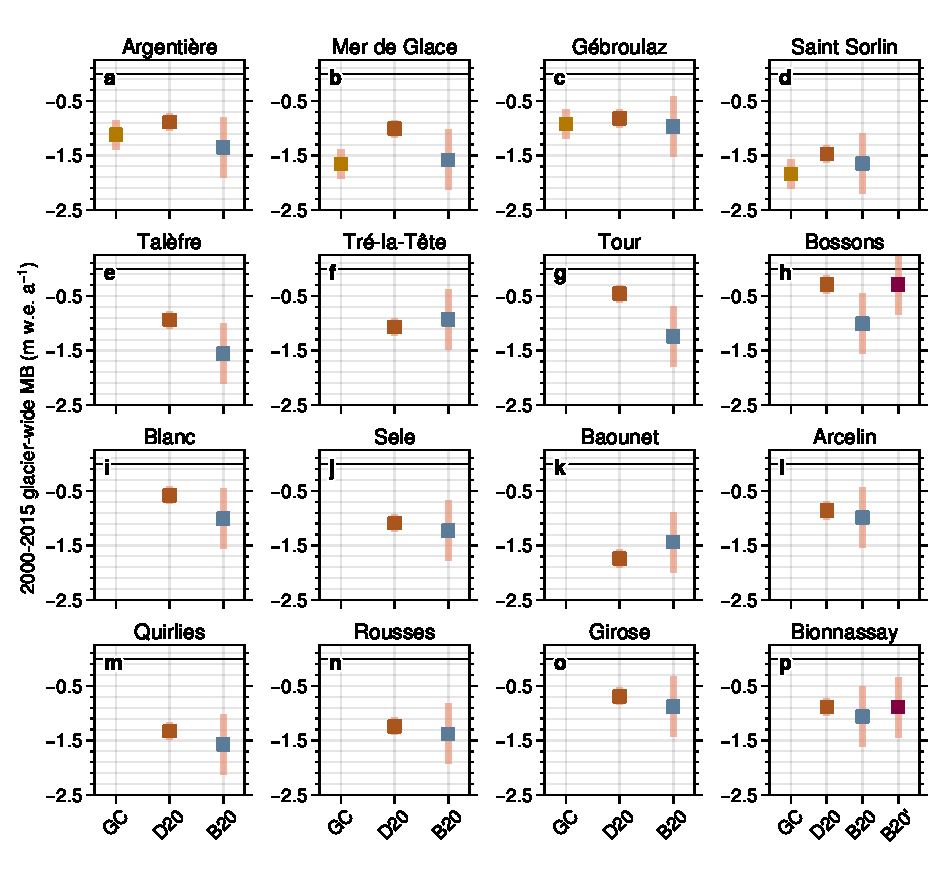
\includegraphics[width=8.3cm]{Figures/intro/Figure_2.pdf}
\caption{Glacierized massifs in the French Alps, with the extent of glaciers for the year 2015.}
\label{intro:fig2}
\end{wrapfigure}

The French Alps are located in the westernmost part of the European Alps, between 44º and 46º13'N and 5.08 and 7.67ºE. Their geographical location amidst the Mediterranean sea and continental Europe produces a particular climate gradient, from south-east to north-west. The southern massifs are more influenced by a Mediterranean climate, receiving less precipitation than their northern counterparts. West Atlantic fluxes bring higher amounts of precipitation to north-western massifs, whereas eastern glaciers close to the Italian border receive most precipitation from east returns \citep{durand_reanalysis_2009}. These different climatic patterns, together with altitudes ranging from sea level to 4810 m at the summit of Mont-Blanc, create an array of sub-climates that influence the evolution of glaciers. A total area of 231 km$^{2}$ was covered by glaciers in the year 2015 the French Alps \citep[with 2015 update]{gardent_multitemporal_2014}.

Like most of the European Alps, the French Alps have been inhabited for many centuries, developing a close relationship between alpine society and mountains. As for mountain peaks, the general social attitude towards glaciers has strongly evolved in the last centuries, transitioning from disdain and terror to awe and curiosity \citep{zryd_les_2008}. During the Little Ice Age, glaciers in the Mont-Blanc massif used to reach the valley, threatening villages and settlements (Fig. \ref{intro:fig3}). During this time, glaciers were regarded as monsters, which were even exorcised to stop their advance \citep{ponchaud_nature_2012}. This relationship between society and glaciers progressively changed in the first half of the 18$^{th}$ century, integrating them as an important cultural elements, thus becoming symbols of identity for alpine societies throughout the European Alps. This means that the loss of glaciers has an additional social consequence in the French Alps, on top of the environmental ones found in all glacierized regions \citep{smit_exploring_2019}. 

These long-term interactions between people and glaciers resulted in some of the earliest studies and observations on glaciers in the world. From the 18$^{th}$ century, the first mountain expeditions were seen as scientific endeavours, providing valuable observations of unknown natural sites \citep{richalet_scientific_2001}. This tradition has continued ever since in the whole European Alps, with the longest observation series of glacier change in the world \citep{glamos_swiss_2019}. In France, the GLACIOCLIM national observatory is now responsible for this task, providing uninterrupted multiple glacier measurements from the field every year since the 1950's. These long-term observations, combined with the rather easy access to glaciers, provide an excellent testbed for glaciological studies. The European and French Alps are some of the regions in the world with a strongest observed glacier mass loss (Fig. \ref{intro:fig1}), a trend that is expected to make them one of the regions with the highest mass loss for this century \citep{marzeion_partitioning_2020}.

\begin{figure*}[h]
\centering
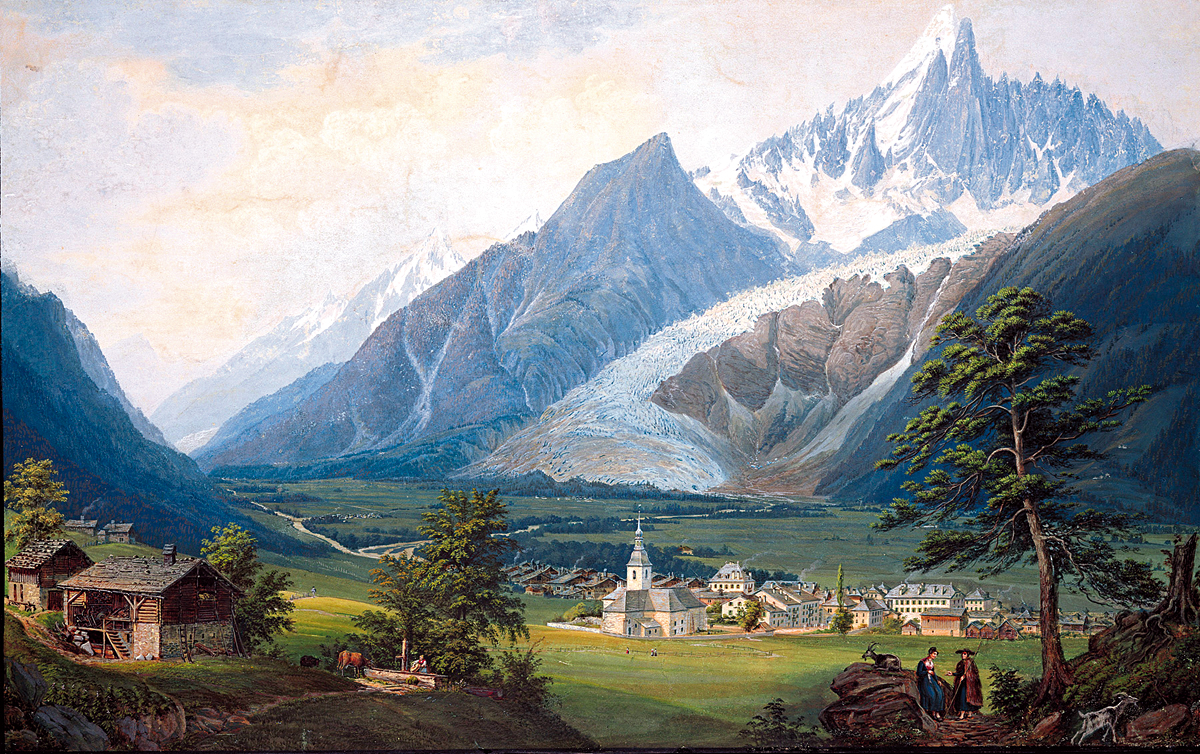
\includegraphics[width=11cm]{Figures/intro/Figure_3.jpg}
\caption{The Mer de Glace in 1822, during the Little Ice Age. By then, its tongue reached the valley, receiving the name of Glacier des Bois, due to the fact that it reached the low-lying forests. \textit{Painting by Jean Dubois}} 
\label{intro:fig3}
\end{figure*}

In many aspects, people in the French Alps have built their lives around mountains and glaciers, whose vast forecasted retreat will impact their socioeconomic model \citep{mourey_evolution_2017, spandre_winter_2019}. Emblematic regions such as the Mont-Blanc massif depend on glaciers for tourism \citep{schut_sport_2013}, water resources and hydropower generation  \citep{laurent_impact_2020}. Moreover, natural hazards derived from glacier retreat might potentially impact populations in valleys \citep{magnin_estimating_2020}. All these effects demand deep changes in the socio-economic model of these regions in order to correctly adapt to these changes in time. This adaptation is impossible without accurate predictions of future glacier evolution. Models can provide answers to these questions, allowing the anticipation and prioritization of actions.

\section{Modelling large-scale glacier evolution}

\emph{"At last, combining the three causes which contribute to the maintenance of glaciers, it would be interesting to arrive at the mass which is supplied to them each year; but one feels that it is only possible to have on this subject more or less probable conjectures; it is especially here that we lack and will always lack observations, which must be the first element to lead to the intelligence of nature."}

Like an oracle, Louis Rendu stated in 1840 in his book "Théorie des glaciers de la Savoie" what all modern glacier modellers are still struggling with \citep{rendu_theorie_1840}. First and foremost, observations are a key element in our understanding of glacier processes. Past observations enable the creation of equations and models to represent in an approximate manner the complex behaviour of glaciers. All glacier models, independently from their approach, will have to solve the two main processes that determine the evolution of glaciers: (a) Glacier mass balance, as the consequence of the mass gained via accumulation (e.g., snowfall, avalanche deposition) and the mass lost through ablation (e.g., ice melting, calving). Mass balance can be seen as the main consequence of climate-glacier interactions \citep{benn_glaciers_2014}; (b) Glacier ice dynamics, that govern the movement of ice downwards due to gravity. Since ice is a viscoelastic material, this movement can occur as a combination of plastic deformation of the ice (also known as creep), sliding of ice over the bed and the deformation of the bed itself \citep{cuffey_physics_2010}. The interplay of mass balance and ice dynamics determines the advance or retreat of glaciers, as a consequence of climate and topography. Past observations of these two main processes have enabled the development of a variety of glacier models of different complexities, used to simulate glacier evolution at different geographical scales. As for any geophysical problem, the larger the study area the more simplifications are used in models. This holds especially for glaciers, for which several parameterizations and simplifications are needed for models to operate at regional or global scale \citep[e.g.,][]{marzeion_past_2012, huss_new_2015, maussion_open_2019}. 

Predicting the future of glaciers is a complex task. It demands a correct representation of past observed glacier changes, accompanied with the hypothesis that the past observed relationships used in the modelling framework will remain constant in the future. This hypothesis would not be necessary with a detailed-enough representation of the physical processes involved in glacier evolution, but a large geographical scale hinders this level of detail in current models. Most importantly, future climate and therefore glacier evolution depend on future anthropogenic greenhouse emissions, introducing large uncertainties in projections that cannot be avoided \citep{marzeion_partitioning_2020}. Therefore, the quest of the modern glacier modeller is to strike a balance between data availability, model complexity and geographical scale.

\section{Teaching machines about glaciers}
\label{intro:ml}

Regional and global glacier evolution models have been developed following a wide variety of approaches. The detailed representation of glacier processes is still a huge challenge, so modellers approach simplifications in different manners. 

The complex physics involved in glacier processes can be simplified using empirical parameterizations, based on assumptions derived from observations. Despite their simplicity, these parameterizations often display a better performance than more complex approaches, since they are well adapted to large-scale problems where some physical processes become less important compared to others \citep{reveillet_relative_2018}. Parameterizations have been applied to both glacier mass balance (e.g., a temperature-index model) and ice dynamics (e.g., area-volume scaling, $\Delta$h parameterization), providing the tools for the vast majority of regional and global glacier evolution models \citep[e.g.,][]{marzeion_past_2012, huss_new_2015, maussion_open_2019, hock_glaciermip_2019}.

Alternatively, statistical models approach simplifications from a purely data-driven perspective. Relationships found in past observations can be used to create statistical models, used to analyse these relationships and performing predictions for unseen cases. Traditional linear statistical models have been applied in glaciology for more than 50 years \citep{hoinkes_glacier_1968, martin_correlation_1974}. In the last decades, statistics have seen a massive increase in both their popularity and research output with the advent of machine learning. The ever-growing amount of data stored by humans is becoming increasingly challenging to use, process and interpret, leading to the development of advanced methods in data science \citep{mjolsness_machine_2001}. As in many research fields, machine learning has  made its way into glaciology (Fig.  \ref{intro:fig3}), albeit with much less intensity than other fields in Earth sciences such as climatology \citep[e.g.,][]{liu_application_2016,ham_deep_2019,jiang_deep_2018} or oceanography \citep[e.g.,][]{ducournau_deep_2016,lguensat_learning_2019}. Linear machine learning models have been applied to regression problems in order to interpret climate-glacier interactions \citep{maussion_enso_2015}, and a shallow neural network was applied to model a glacier's mass balance and length \citep{steiner_application_2005,steiner_sensitivity_2008}. 

\encart{The "black box" effect}{Machine learning is a relatively new research field, with a lot of complicated jargon that is in constant evolution due to the high research output of the last years. This rapid evolution, often displaying rather spectacular results in particular applications, has nonetheless been counterbalanced by a reputation that machine learning models act essentially as "black boxes". They are regarded as opaque models, taking input data, training on them in order to reproduce the patterns in the dataset, and spitting out the results without the possibility of understanding what is going on inside them. While this might be true for certain situations, this general statement is quite misleading, and it can be the source of a great deal of confusion. Deep learning, being a particular family of machine learning, can often act as a black box as I am going to show in this work, but this is not the case for many other algorithms. The so-called "accuracy \textit{vs} interpretability" tradeoff tells us that, as a rule of thumb, methods with the strongest predictive power are also the most complex ones to interpret. Therefore, machine learning can still be used to interpret relationships in data, at the cost of sacrificing some predictive power \citep{riccia_machine_1997}. Nonetheless, this notion is currently being challenged by a new wave of interpretable machine learning methods, spearheaded by interpretable deep learning \citep[e.g.,][]{dong_improving_2017, zhang_interpretable_2018, rackauckas_universal_2020}. These new methods, as I am going to elaborate in the last chapter, have a huge potential to overcome the current limitations of machine learning.}

In the last years, neural networks have been revolutionized with new methods enabling the training of deep neural networks (i.e. deep learning), composed of multiple intermediate layers. This depth allows the neural networks to capture more complex non-linear patterns in data, resulting in improved performance in a wide range of problems \citep{wang_origin_2017}. Nonetheless, very few efforts have been made in this direction in glaciology in the recent years, with most recent research focusing on classification problems \citep{mohajerani_detection_2019, baumhoer_automated_2019, zhang_automatically_2019}. Classification problems offer a more straightforward problem to validate in geosciences, avoiding the tricky question of reproducing physical processes with a "black box" approach \citep{karpatne_theory-guided_2017}. Applying deep learning to geophysical regression problems is a complex task, demanding a solid validation of the results in order to avoid pitfalls related to spatiotemporal data independence \citep{roberts_cross-validation_2017}. 

In this manuscript, I introduce my attempt to apply deep learning to model glacier evolution at a regional scale. The French Alps are used as a case study, for which their evolution is studied from the late 1960's until the end of the 21$^{st}$ century. As it often happens in science, this investigation on deep learning was not included in my original PhD project. Initial tests with a simple statistical glacier mass balance model slowly evolved into more complex linear machine learning and eventually into deep learning. A great deal of what is included in this manuscript are the lessons learnt from numerous problems, mistakes and dilemmas that I encountered during these three years. 

\begin{figure*}[h]
\centering
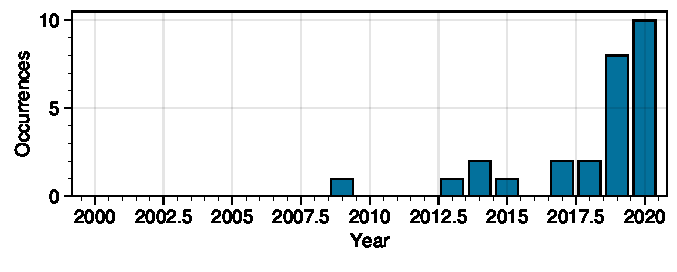
\includegraphics[width=11cm]{Figures/intro/Figure_4.pdf}
\caption{Number of scientific articles containing the words "glacier machine learning", based on queries on Web of Science.}
\label{intro:fig4}
\end{figure*} 

\section{Modelling glacierized mountain catchments}

The correct assessment of the consequences of glacier retreat requires not only an understanding of the evolution of glaciers, but a hydro-ecological perspective of their role at the catchment scale. In the French Alps, this type of studies are only found at the scale of the whole European Alps \citep{coppola_impact_2018} or the Mont-Blanc massif \citep{laurent_impact_2020}. The J2K hydrological model \citep{krause_quantifying_2002}, developed at the University of Jena (Germany), has been applied and co-developed for many years by hydrologists in many countries, including France, in a wide variety of catchment configurations \citep{branger_investigating_2012, braud_j2000-rhone_2017, horner_information_2020}. Among these studies, a special focus was placed in glacierized catchments, with a few glacio-hydrological modelling studies in Himalayan mountain catchments \citep{gao_test_2012, nepal_understanding_2014}. The current representation of glaciers in J2K takes into account a wide variety of processes, including snow accumulation, sublimation, ageing and melt; and ice melt under different condition including debris covers \citep{nepal_understanding_2014}. Nonetheless, the absence of glacier geometry evolution hinders its application for long-term projections in glacierized mountain catchments. Indeed, in the current version of J2K, glaciers are included as static objects, acting as unchanging ice reservoirs \citep{nepal_understanding_2014}. This approach is highly problematic in the current context of rapid glacier retreat.  Other hydrological models in France (e.g., GR rainfall-runoff models, \cite{coron_suite_2017}) suffer from a lack of representation of glaciers, highlighting the gap in knowledge on the fate of glacierized catchments in the French Alps. 

In this manuscript, I introduce an attempt to solve this problem, using output data from a glacier evolution model developed during this project \citep{bolibar_alpgm_2020}, in order to take into account glacier evolution in the J2K hydrological model. The initial objective of my PhD was to correctly assess the future glacio-hydrological changes in the French Alps and the whole Rhône river catchment. It combined a first part on regional glacier modelling with a second part about glacio-hydrological modelling at the scale of the whole Rhône river catchment. This initial objective was driven by the BERGER project funded by the Auvergne-Rhône-Alpes region. This project, which partially funded my PhD work, aims at understanding the impacts of future glacier retreat in the French Alps on aquatic communities living in glacier-fed streams. By providing accurate estimates of future glacier evolution and glacier runoff, ecologists will be able to extrapolate how changes in runoff intensity, water temperature and seasonality might affect these communities \citep{robinson_ecosystem_2014, cauvy-fraunie_global_2019}. Due to the unexpected turn of events during the three years of this project, a great fraction of the time was focused on machine learning applications for glacier evolution modelling (Sect. \ref{intro:ml}). This impacted the original objectives, leaving less time to work on regional glacio-hydrological modelling. Therefore, efforts on glacio-hydrological modelling have been focused on a technical implementation of glacier dynamics in a well-documented glacierized catchment, and the assessment of glacier retreat and its hydorlogical effects over the recent past. This work provides a validated novel methodology, ready to be applied at a larger geographical scale in future studies.

\section*{Objectives of this PhD work}
\addcontentsline{toc}{chapter}{Objectives of this PhD work}

The work of my PhD has contributed to two main research axes: (a) the methods, where I introduce a first effort to apply deep learning to model glacier evolution at a regional scale, and the addition of glacier evolution into a process-based hydrological model; (b) the results, where I analyse and present the results of numerical simulations of the evolution of all glaciers in the French Alps from the late 1960's to the end of the 21$^{st}$ century. With the combination of these two axes I attempt to address the following scientific questions:
 
\begin{list}{\textbf{Question}}{}

\item \textbf{1} - Can deep learning be applied to model annual glacier mass balance changes at a regional scale? What are the benefits of using nonlinear deep learning models compared to linear machine learning?

\item \textbf{2}  - What are the annual glacier changes of all glaciers in the French Alps for the last half century? 

\item \textbf{3} - How will French alpine glaciers evolve during the 21$^{st}$ century? How does glacier retreat affect the climate signal on glaciers? What are the main factors that determine glacier survival in the French Alps?

\item \textbf{4} - What are the current limitations in the representation of glaciers in hydrological models in France? How can this be improved?

\end{list}

After answering these questions during this work, a new one arose, setting the direction of future research venues:

\begin{list}{\textbf{Question}}{}

\item \textbf{5} - What are the caveats of the deep learning modelling approach used in this work? What improvements are needed to overcome these limitations for glaciological studies?

\end{list}

\section*{A short note to the reader}
\addcontentsline{toc}{chapter}{A short note to the reader}

This manuscript consists of three parts: one dedicated to regional glacier evolution modelling, another one to glacio-hydrological modelling of glacierized alpine catchments and a final one as an outlook. Part I, being the largest one, is built around three papers: two published and one in preparation. Each paper is included as a dedicated chapter, with a small preface giving the necessary context to the reader. This regional glacier modelling part follows a logical structure found in most publications: a first paper dedicated to the methods (Chapter 2), a second paper dedicated to the results of the application of this method to reconstruct past mass balance changes in the French Alps (Chapter 3), and a third paper dedicated to the future evolution of French alpine glaciers under different scenarios of climate change (Chapter 4). Part II, dedicated to glacio-hydrological modelling of glacierized catchments, is included as a single chapter (Chapter 5) with a section detailing the modelling approach, and a results section presenting the preliminary results. At last, Part III, with Chapter 6, serves as a conclusion, where various relevant topics of this manuscript are discussed and some perspectives are laid down regarding the most promising future research venues of this work.